\section{Lezione del 27 novembre}
Quello che possiamo dire riguardo a una rete causale, è che registra il comportamento di un sistema elementare.\\
All'interno della rete si hanno quindi, con i tagli, possibili ose e solo servazioni di configurazioni possibili nella storia del sistema.\\
Grazie alle reti causali $N=(B,E,F)$, preso un elemento $x\in X$, possiamo definire:
\begin{itemize}
    \item \textbf{past(x)}, ovvero il passato dell'elemento, tutti gli elementi in relazione $\leq$ di $x$
    \item \textbf{future(x)}, ovvero il futuro dell'elemento, tutti gli elementi in relazione $\geq$ di $x$
\end{itemize}
    Visualizzabili, per esempio, nell'immagine, rispettivamente in rosso e blu:
    \begin{figure}[H]
    \centering
    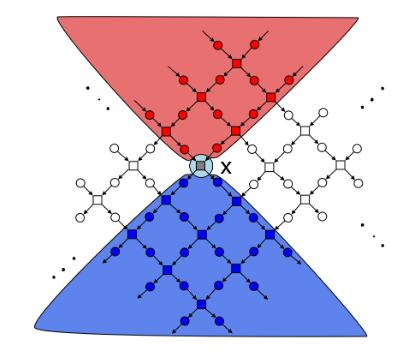
\includegraphics[scale = 0.5]{IMM/cono_di_luce.jpg} 
    \end{figure}
Gli elementi nell'anti-cono (la parte bianca) sono in relazione \textbf{co} con $x$ e quindi possono ese e solo sere concorrenti.

\subsection{k-densità}
Data una rete causale $N=(B,E,F)$ e dato un ordine parziale $(X, \leq)$ con $X=B\cup E$ definiamo che la rete è \textbf{K-densa} se ogni linea ed ogni taglio si intersecano in un punto, tutti hanno un punto comune. Formalmente: \[\forall\,h\in Linee(N),\forall\,c\in Tagli(N):|h\cap c|=1\] Con $Linee(N)$ e $Tagli(N)$ che sono rispettivamente gli insiemi di tutte le linee e dei tagli. Se $N$ è finita è anche \textbf{K-densa}, se sono infinite non è detto.\\

Sia $\Sigma=(S,T,F,c_{in})$ un sistema elementare senza contatti e finito, tale che $S\cup T$ sia finito. Si ha che, con $\phi$ che mappa dalla rete causale al sistema elementare, $\langle N=(B,E,F), \phi\rangle$ è un processo non sequenziale di $\Sigma$ se e solo se:
\begin{itemize}
    \item $(B,E,F)$ è una rete causale dove si ammettono anche condizioni isolate
    \item $\phi:B\cup E \to S\cup T$ è una mappa tale che:
    \begin{itemize}
      \item $\phi(B)\subseteq S, \phi(E)\subseteq T$, far corrispondere alle condizioni, condizioni del sistema, e ad eventi eventi del sistema. 
      \item $\forall x,y\in B\cup E:\phi(x)=\phi(y)\implies (x\leq y)\lor (y\leq x)$, se due elementi della rete corrispondo allo stessa condizione del sistema, questi eventi sono successive occorrenze di quel elemento e quindi nella rete causale sono sicuramente ordinati, non si ha quindi concorrenza
      \item $\forall e\in E:\phi(\,^\bullet e)=\,^\bullet \phi(e)\land\phi(e^\bullet)=\phi(e)^\bullet$ quindi le precondizioni di un evento nella rete causale devono corrispondere alle pre condizioni dell'immagine dell'evento nel sistema elementare (e così anche per le post)
      \item $\phi(Min(N))=c_{in}$, con $Min(N)=\{x\in B\cup E|\nexists y \mbox{tale che }(y,x)\in F\}$, ovvero se vado a prendere gli elementi minimali della rete causali, ovvero tutti quei elementi che non hanno un arco entrante, questi vengono mappati nel caso iniziale del sistema elementare.
    \end{itemize}
\end{itemize}
Se ho queste proprietà la rete causale è una registrazione del sistema elementare.\\ 
In tal caso si ha che $N=(B,E,F)$ è K-densa (sia che sia finita che infinita), avendo il sistema di partenza finito. Le linee sono quindi sottoprocessi sequenziali e i tagli possibili configurazioni sempre raggiungibili.\\ Inoltre si ha che:
\[\forall K \subseteq B, K\mbox{ è B-taglio di } N \mbox{ tale che } K \mbox{ è finito} \land \exists c\in C_\Sigma:\phi(K)=c\] 
Quindi i tagli fatti di condizioni corrispondono a casi raggiungibili. Due punti non possono essere sia in relazione \textbf{co} che in relazione \textbf{li}. Se la retta è dimostrabile essere finita, allora questa è \textbf{k-densa}.\\

Dato un sistema ho tanti processi non sequenziali che rappresentano esecuzioni del sistema. Ci si chiede quindi se ho un unico oggetto che rappresenta tutti i possibili run del sistema.

